%%%%%%%%%%%%%%%%%%%%%%%%%%%%%%%%%%%%%%%%%
% Beamer Presentation
% LaTeX Template
% Version 1.0 (10/11/12)
%
% This template has been downloaded from:
% http://www.LaTeXTemplates.com
%
% License:
% CC BY-NC-SA 3.0 (http://creativecommons.org/licenses/by-nc-sa/3.0/)
%
%%%%%%%%%%%%%%%%%%%%%%%%%%%%%%%%%%%%%%%%%

%----------------------------------------------------------------------------------------
%	PACKAGES AND THEMES
%----------------------------------------------------------------------------------------

\documentclass{beamer}

\mode<presentation> {
	
	% The Beamer class comes with a number of default slide themes
	% which change the colors and layouts of slides. Below this is a list
	% of all the themes, uncomment each in turn to see what they look like.
	
	%\usetheme{default}
	%\usetheme{AnnArbor}
	%\usetheme{Antibes}
	%\usetheme{Bergen}
	%\usetheme{Berkeley}
	%\usetheme{Berlin}
	%\usetheme{Boadilla}
	%\usetheme{CambridgeUS}
	%\usetheme{Copenhagen} %nice
	\usetheme{Darmstadt} %small subsection name on top
	%\usetheme{Dresden}
	%\usetheme{Frankfurt} %need to specify frametitle
	%\usetheme{Goettingen}
	%\usetheme{Hannover}
	%\usetheme{Ilmenau}
	%\usetheme{JuanLesPins}
	%\usetheme{Luebeck}
	%\usetheme{Madrid} %standard
	%\usetheme{Malmoe}
	%\usetheme{Marburg}
	%\usetheme{Montpellier}
	%\usetheme{PaloAlto}
	%\usetheme{Pittsburgh}
	%\usetheme{Rochester}
	%\usetheme{Singapore}
	%\usetheme{Szeged}
	%\usetheme{Warsaw}
	
	% As well as themes, the Beamer class has a number of color themes
	% for any slide theme. Uncomment each of these in turn to see how it
	% changes the colors of your current slide theme.
	
	%\usecolortheme{albatross}
	%\usecolortheme{beaver}
	%\usecolortheme{beetle}
	%\usecolortheme{crane}
	%\usecolortheme{dolphin}
	%\usecolortheme{dove}
	%\usecolortheme{fly}
	%\usecolortheme{lily}
	%\usecolortheme{orchid}
	%\usecolortheme{rose}
	%\usecolortheme{seagull}
	%\usecolortheme{seahorse}
	%\usecolortheme{whale}
	%\usecolortheme{wolverine}
	
	%\setbeamertemplate{footline} % To remove the footer line in all slides uncomment this line
	%\setbeamertemplate{footline}[page number] % To replace the footer line in all slides with a simple slide count uncomment this line
	
	%\setbeamertemplate{navigation symbols}{} % To remove the navigation symbols from the bottom of all slides uncomment this line
}

\usepackage{graphicx} % Allows including images
\usepackage{booktabs} % Allows the use of \toprule, \midrule and \bottomrule in tables
\usepackage{sansmathaccent}
\pdfmapfile{+sansmathaccent.map}
\usepackage{comment} %comment
%----------------------------------------------------------------------------------------
%	TITLE PAGE
%----------------------------------------------------------------------------------------

\title[Master Thesis]{Applying Machine Learning to LTE/5G Performance Trend Analysis} % The short title appears at the bottom of every slide, the full title is only on the title page

\author{Araya Eamrurksiri}
\institute[LiU] % Your institution as it will appear on the bottom of every slide, may be shorthand to save space
{
	Linkoping university \\ % Your institution for the title page
	\medskip
	\textit{} % Your email address
}
\date{June 2, 2017}

\begin{document}
	
	\begin{frame}
	\titlepage % Print the title page as the first slide
\end{frame}

%\begin{frame}
%\frametitle{Overview} % Table of contents slide
%\tableofcontents 
%\end{frame}

%----------------------------------------------------------------------------------------
%	PRESENTATION SLIDES
%----------------------------------------------------------------------------------------

\section{Introduction} 
\subsection{Motivation}
\begin{frame}
%\frametitle{Motivation}

\begin{itemize}
	\item Many test cases are executed for testing software packages 
	\item Evaluate the performance of an updated software package by visualizing the graph 
	\item Algorithm that can reduce workload of manual inspection
\end{itemize}	

\end{frame}
%------------------------------------------------
\subsection{Objectives}
\begin{frame}
%\frametitle{Objectives}
\begin{itemize}
\item Detect the state of the CPU utilization (degrading, improving, or steady state)
\item Detect whether there is any change in the test environment that affects the CPU utilization
\end{itemize}
\end{frame}

%------------------------------------------------
\section{Data}
\subsection{Data sources}
\begin{frame}[fragile]
%\frametitle{Data sources}
\begin{comment}
Software release 
\begin{itemize}
\item two major releases per year
\item labeled with L followed a number related to the year of release and a letter A or B
\end{itemize}

Software package
\begin{itemize}
\item act as a snapshot or marker
\item labeled with R followed numbers and letters
\end{itemize}
\end{comment}

\begin{itemize}
\item Software release
\item Software package - treated as a \textit{time point} in the time series data
\item Test cases \footnotesize{in QA capacity area on signaling capacity} \normalsize{- treated as an \textit{observation} in the dataset}

%\begin{figure}
%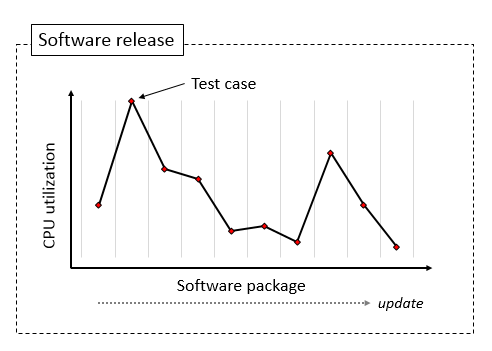
\includegraphics[width=0.6\linewidth]{data-structure}
%\caption{An example of the CPU utilization value in each software package from one software release}
%\end{figure}

\end{itemize}

\end{frame}


%------------------------------------------------
\subsection{Data preprocessing}
\begin{frame}
%\frametitle{Data preprocessing}
Data is collected on January 20, 2017

Three datasets: Software release A, B, and C
\begin{itemize}
\item Sorted by software package version
\item Filtered out test cases which are not executed properly
\item Selected test case which has the \textit{lowest} value of the CPU utilization to represent a performance of a specific software package
\end{itemize}

In total, each dataset contains 64, 241, and 144 test cases, respectively

\end{frame}

%------------------------------------------------
%\begin{frame}
%EventsPerSec: Event intensity 
%\begin{itemize}
%	\item Contains several \textit{local events}
%	\item Stores multiple values separated by a tab character
%	\item Some local events are used as predictor variables
%	\item Implement a function to split each element to columns
%\end{itemize}
%
%\end{frame}

%------------------------------------------------
\begin{frame}
Response variable 
\begin{itemize}
\item TotCpu\%: CPU utilization
\end{itemize}	
\vspace{1em}
Predictor variables
\begin{itemize}
\item local events in EventsPerSec
\begin{itemize}
\item RrcConnectionSetupComplete
\item Paging
\item X2HandoverRequest
\end{itemize}	
\item Test environments
\begin{itemize}
\item DuProdName: Product hardware name
\item Fdd/Tdd: Different standard of LTE 4G Technology
\item NumCells: Number of cells in the base station
\end{itemize}
\end{itemize}

\end{frame}

%------------------------------------------------
\section{Method} 
\begin{frame}
Method 
\begin{itemize}
\item Markov switching model
\item E-divisive method
\item Tools
\end{itemize}
\end{frame}
%------------------------------------------------
\subsection{Markov switching model}
\begin{frame}

\begin{block}{Markov switching autoregressive model}
\[
y_{t} = X_{t}\beta_{S_{t}} + \phi_{1,S_{t}} y_{t-1} + \varepsilon_{t}, \quad \varepsilon_{t} \sim N(0,\sigma^{2}_{S_{t}})
\]
\end{block}

Assuming that $S_{t}$ denote an unobservable state variable

$y_{t}$ is the observed value of time series at time $t$ 

$X_{t}$ is a design matrix containing the predictor variables of time series at time $t$ 

$\beta_{S_{t}}$ are a column vector of the coefficients in state $S_{t}$, where $S_{t}=1,2,...,k$

$\phi_{1,S_{t}}$ is an autoregression coefficient at time $t-1$ in state $S_{t}$

%\begin{figure}
%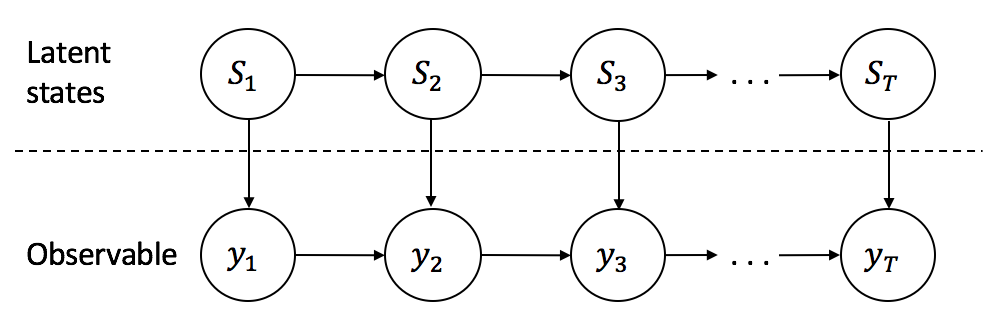
\includegraphics[width=0.5\linewidth]{msm-ar1}
%\caption{Model with additional dependencies at observation level}
%\end{figure}

\end{frame}

%------------------------------------------------
\begin{frame}

\begin{block}{Markov switching autoregressive model}
\[
y_{t} = X_{t}\beta_{S_{t}} + \phi_{1,S_{t}} y_{t-1} + \varepsilon_{t}, \quad \varepsilon_{t} \sim N(0,\sigma^{2}_{S_{t}})
\]
\end{block}

Assuming that $S_{t}$ denote an unobservable state variable

\vspace{1em}

A coefficient of a predictor variable can have either different values in different state, $\beta_{S_{t}}$,  or a constant value in all state, $\beta$. 

\vspace{1em}

The variable whose coefficient can take on \textit{different} values is said to have a \textbf{switching effect}. 

\vspace{1em}

The variable which has the \textit{same} coefficient in all states is the variable that does not have a switching effect, or said to have a \textbf{non-switching effect}. 
\end{frame}

%------------------------------------------------
\subsection{E-divisive method}
\begin{frame}[fragile]

\begin{comment}
E-divisive method \cite{p3}
\begin{itemize}
\item Non-parametric approach: more flexible as no assumption about the distribution is made
\item Detects multiple change point locations based on a divisive hierarchical estimation algorithm
\item Algorithm: Recursively partition a time series, and perform a permutation test to find the statistical significance of an estimated change point.
\item Remark: Obtain a rough idea of the change point location 
\end{itemize}

\begin{figure}
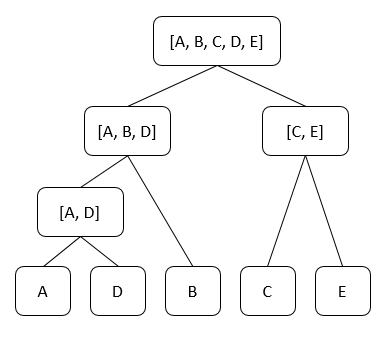
\includegraphics[scale=0.3]{divisive}
\end{figure}
\end{comment}

\begin{columns}[c] % The "c" option specifies centered vertical alignment while the "t" option is used for top vertical alignment

\column{.65\textwidth} % Left column and width
E-divisive \cite{p3}
\begin{enumerate}
\item Non-parametric approach: more flexible as no assumption about the distribution is made
\item Detects multiple change point locations based on a divisive hierarchical estimation algorithm
\item Algorithm: Recursively partition a time series, and perform a permutation test to find the statistical significance of an estimated change point.
\item Remark: Obtain a rough idea of the change point location 
\end{enumerate}

\column{.35\textwidth} % Right column and width
%\begin{figure}
%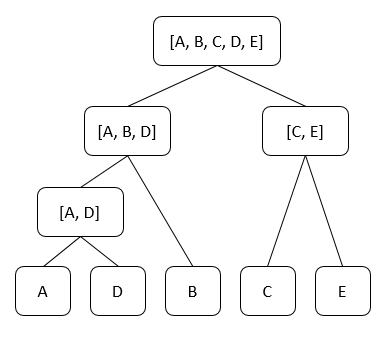
\includegraphics[width=1\linewidth]{divisive}
%\caption{Divisive hierarchical clustering}
%\end{figure}

\end{columns}

\end{frame}
%------------------------------------------------
\subsection{Tools}
\begin{frame}
\texttt{R} programming

\begin{itemize}
\item Markov switching model is performed using \textit{MSwM} package \cite{p2}

Various extensions and modifications were made in the package

For example, 

$\quad \rightarrow$ Make it more stable to use with categorical variables

$\quad \rightarrow$ State prediction function

$\quad \rightarrow$ Plot for visualizing the results

\item E-divisive method is performed using \textit{ecp} package \cite{p3}
\end{itemize}

\end{frame}

%------------------------------------------------
\section{Results and Discussion}

\begin{frame}
Results and Discussion

\begin{itemize}
\item Markov switching model
\begin{itemize}
\item Analysis I: Number of state
\item Analysis II: Number of switching coefficients
\end{itemize}

\item E-divisive method
\item Comparison between both methods
\begin{itemize}
\item Simulated data
\item Real data
\end{itemize}

\item State inference on the results from the Markov switching model
\end{itemize}

\end{frame}
%------------------------------------------------
\subsection{Markov switching model}
\begin{frame}
When applying the Markov switching model, we need to decide on
\begin{itemize}
\item Number of states, $k$
\item Number of switching coefficients in the model
\end{itemize}
\vspace{1em}

Based on the applied literature, the information criteria called the Bayesian Information Criterion (BIC) is used for model selection

$$\mathrm{BIC}=-2\ln(L(\hat{\theta}))+m\cdot\ln(T)$$

\footnotesize{where, $m$ is the number of parameters and $T$ is the number of observations}
\vspace{1em}

\normalsize{BIC attempts to reduce an overfitting problem by penalizing on the number of parameters in the model}

\end{frame}

%------------------------------------------------
%\subsection{Markov switching model}
\begin{frame}

Analysis I: Number of states

Hypothesis: Markov switching model with \textit{two} or \textit{three} states
\rule{\textwidth}{0.4pt}

\begin{itemize}
\item Model with lower BIC value is preferable
\item However, model output along with plot should also be taken into account as well
\pause
\item Two-state model offered less details, and plots were unrealistic and difficult to make an interpretation
\item \textbf{Three-state} model was chosen for further analysis as it provided more intepretable plots and better fit
\item \small{Remark: Higher number of states $k\geq4$ are more likely to give worse results and were not considered}
\end{itemize}

\end{frame}

%------------------------------------------------
%\subsection{Markov switching model}
\begin{frame}[fragile]
Analysis II: Number of switching coefficients in the model

Hypothesis: Test environments (\textit{DuProdName}, \textit{Fdd/Tdd}, and \textit{Numcells}) is possible to have non-switching effects
\rule{\textwidth}{0.4pt}

\begin{itemize}
\item \small{\textit{Recall: The variable whose coefficient is \textit{constant} in all states are said to have a non-switching effect}}

\item \normalsize{Attempt to reduce the number of parameters to be estimated in the model
\item Algorithm used numerical optimization

$\rightarrow$ more estimated parameters will make the obtained result unstable 

\item Each dataset of the software release was tested with different models
\item Three final models for each dataset were obtained}
\end{itemize}


\begin{comment}
\begin{itemize}
\item Software release L16A: 

\textit{Fdd/Tdd} and \textit{Numcells} are non-switching coefficients

\item Software release L16B: 

\textit{DuProdName} is non-switching coefficient


\item Software release L17A: 

\textit{DuProdName}, \textit{Fdd/Tdd}, and \textit{NumCells} are non-switching coefficients
\end{itemize}
\end{comment}

\begin{comment}
Software release L16A

Model with Fdd/Tdd and Numcells are non-switching coefficients

\begin{figure}
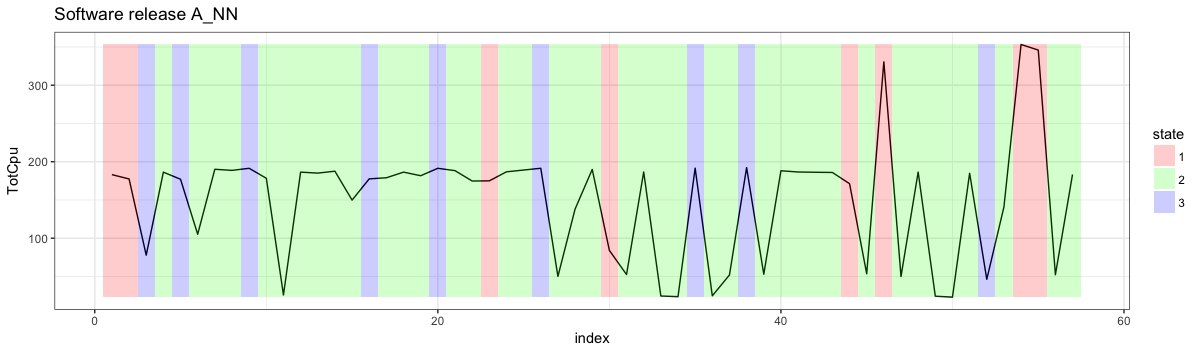
\includegraphics[width=1\linewidth]{L16A_NN1}
\caption{The CPU utilization showing the periods where the observation is in the specific state.}
\end{figure}


\small{Decide: Number of switching coefficients in the model

Hypothesis: test environments is possible to have non-switching effects}
\rule{\textwidth}{0.4pt}

Software release L16B

Model with DuProdName is non-switching coefficient.

\begin{figure}
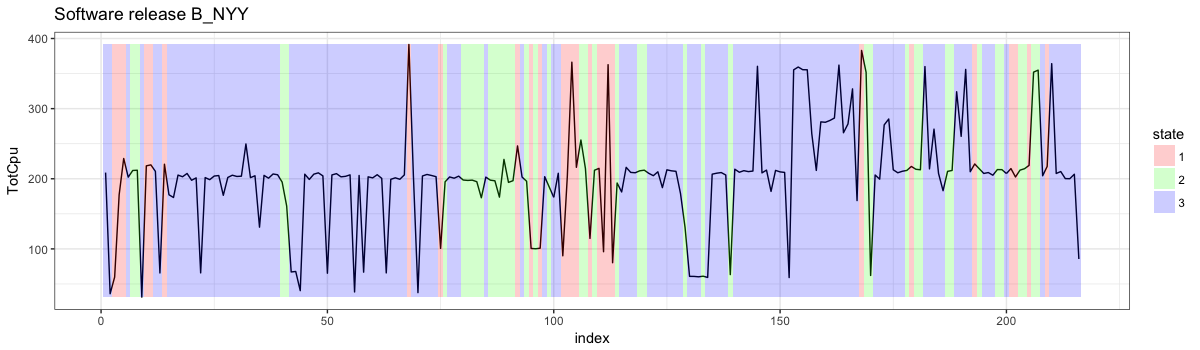
\includegraphics[width=1\linewidth]{L16B_NYY1}
\caption{The CPU utilization showing the periods where the observation is in the specific state.}
\end{figure}


\small{Decide: Number of switching coefficients in the model

Hypothesis: test environments is possible to have non-switching effects}
\rule{\textwidth}{0.4pt}


Software release L17A

Model with DuProdName, Fdd/Tdd, and NumCells are non-switching coefficients.

\begin{figure}
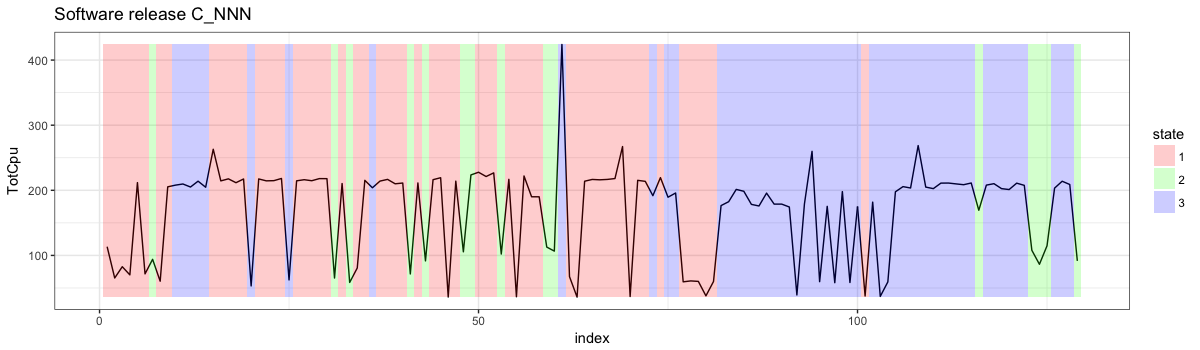
\includegraphics[width=1\linewidth]{L17A_NNN1}
\caption{The CPU utilization showing the periods where the observation is in the specific state.}
\end{figure}
\end{comment}

\end{frame}

%------------------------------------------------
\subsection{E-divisive}
\begin{frame}

\begin{itemize}
\item Apply the E-divisive method to all three datasets of the software release L16A, L16B, and L17A
\item Input: the value of the CPU utilization
\end{itemize}

\end{frame}

%------------------------------------------------
\subsection{Simulation study for model evaluation}
\begin{frame}
\begin{itemize}
\item In the real data, the state of the CPU utilization is unknown $\rightarrow$ Evaluation of the model can't be made
\pause
%\vspace{1em}

\item Simulated two datasets (Dataset 1 and Dataset 2) with the ground truth about the state. 

The real models for each state are
\end{itemize}

$y_{t}=\begin{cases}
\begin{array}{c}
10+0.6X_{1,t}-0.9X{}_{2,t}+0.5y_{t-1}+\varepsilon_{t}^{(1)}\\
2+0.8X_{1,t}+0.2y_{t-1}+\varepsilon_{t}^{(2)}\\
-12+0.7X_{1,t}+0.2X{}_{2.t}-0.2y_{t-1}+\varepsilon_{t}^{(3)}
\end{array} & \begin{array}{c}
\mathrm{Normal}\\
\mathrm{Bad}\\
\mathrm{Good}
\end{array}\end{cases}$
\vspace{1em}

$y_{t}$ is assumed to be value of a CPU usage

$x_{1,t}\sim U[50,200]$

$x_{2,t}\sim U[0,50]$ 

$\varepsilon_{t}^{(1)}\sim N(0,1),\quad \varepsilon_{t}^{(2)}\sim N(2,0.5),\quad \mathrm{and} \quad \varepsilon_{t}^{(3)}\sim N(1,1)$

\end{frame}

%------------------------------------------------
\begin{frame}

\begin{figure}
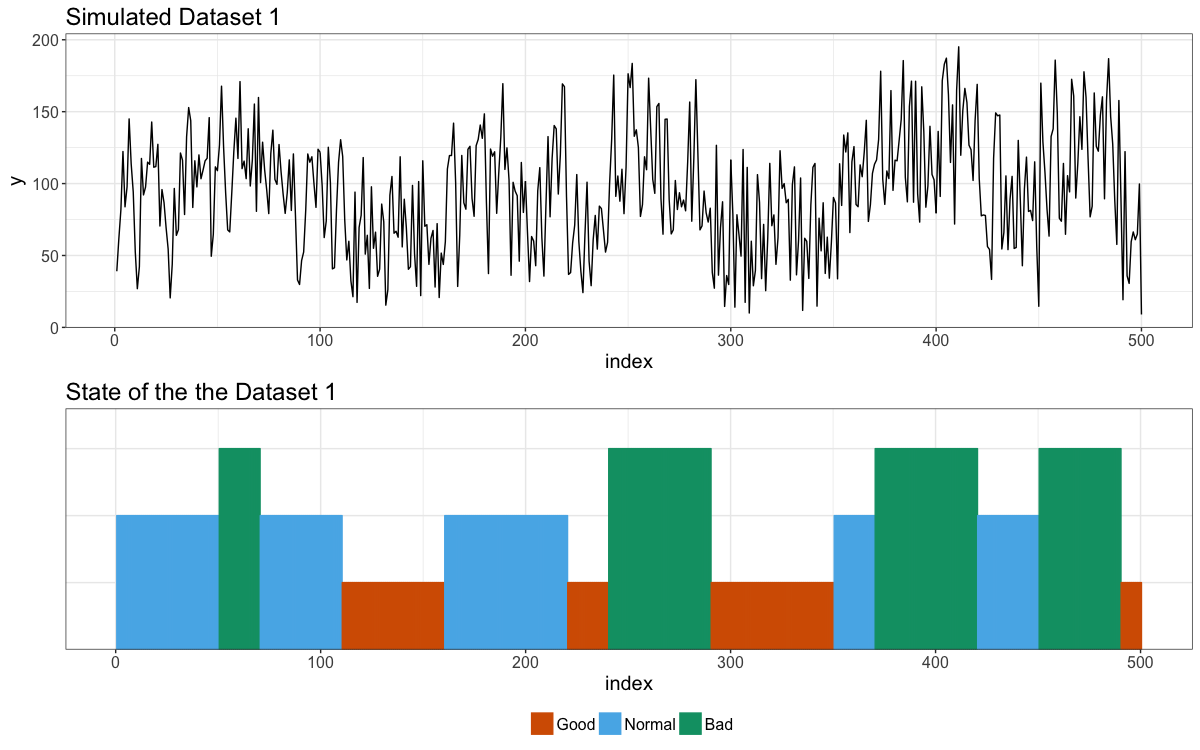
\includegraphics[width=1\linewidth]{sim1}
\caption{A simulated data of Dataset 1 and the period in the time series when observation is in each state.}
\end{figure}

\end{frame}

%------------------------------------------------
\begin{frame}

\begin{figure}
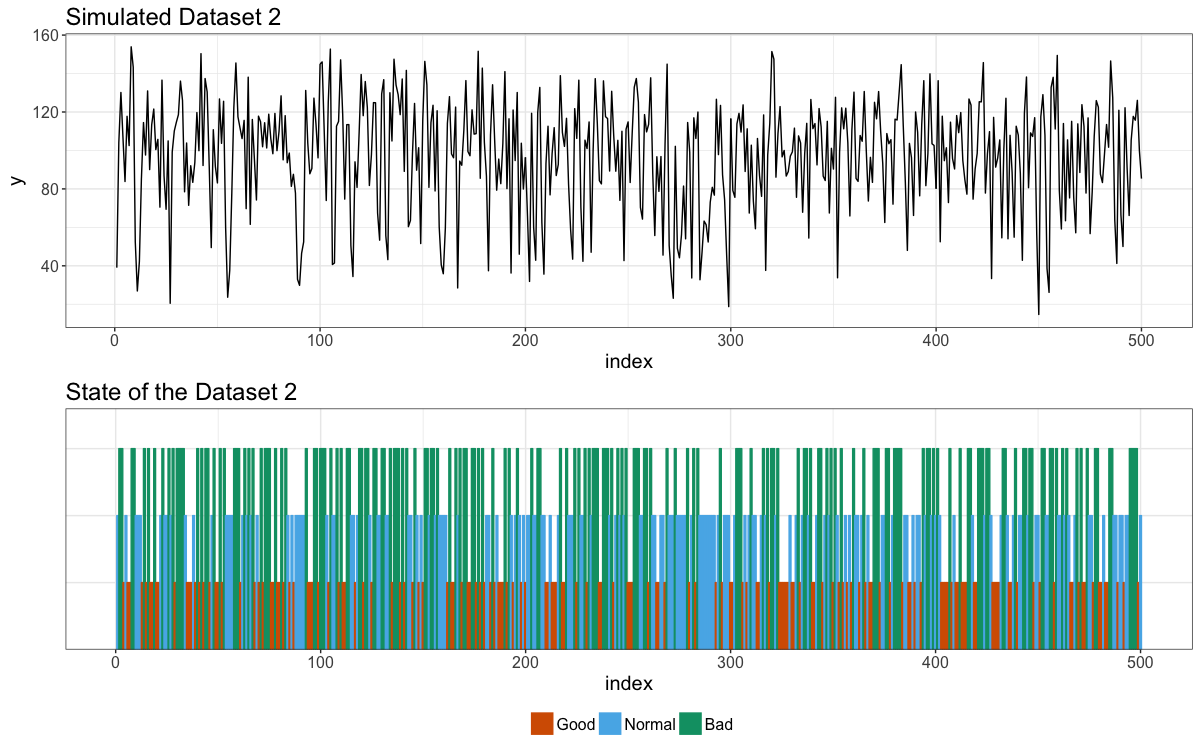
\includegraphics[width=1\linewidth]{sim2}
\caption{A simulated data of Dataset 2 and the period in the time series when observation is in each state.}
\end{figure}

\end{frame}

%------------------------------------------------
\subsection{Comparison between both methods}
\begin{frame}[fragile]
Apply the Markov switching model and the E-divisive method to the simulated Dataset 1 and Dataset 2, it is found that
\pause

\begin{itemize}
\item Both methods detect changes at the same location 

$\rightarrow$ high probability to be an actual change

\item Both methods detect changes close to one another but not at the exact location 

$\rightarrow$ lower chance to be a false alarm
\end{itemize}


\begin{comment}
\begin{figure}
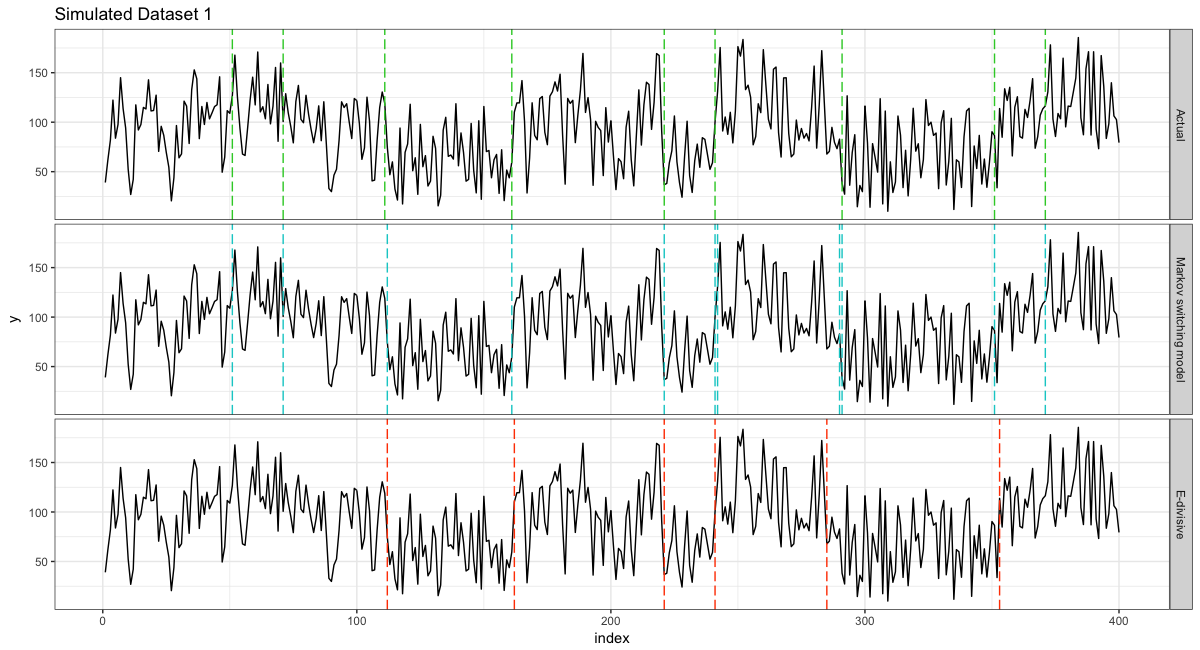
\includegraphics[width=1\linewidth]{compare_sim1}
\caption{The simulated Dataset 1 showing the estimated change point locations}
\end{figure}

Simulated Dataset 2

\begin{figure}
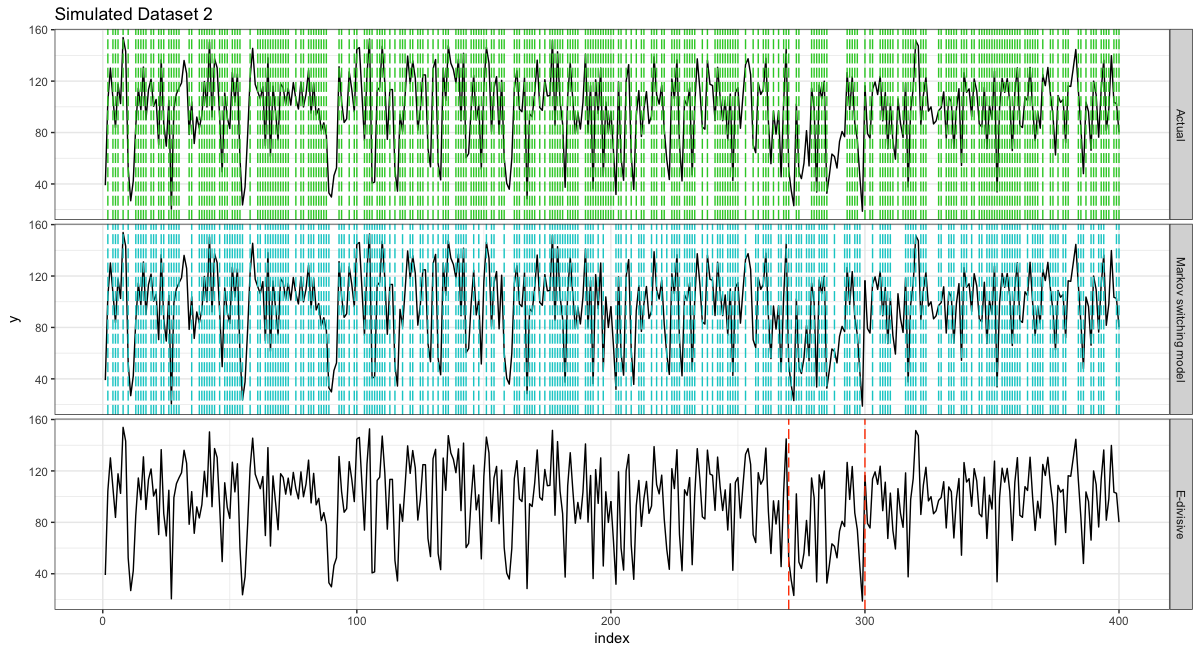
\includegraphics[width=1\linewidth]{compare_sim2}
\caption{The simulated Dataset 2 showing the estimated change point locations}
\end{figure}
\end{comment}

\end{frame}

%------------------------------------------------
\begin{frame}
Real data: Software release A

\begin{itemize}
\item E-divisive cannot detect any changes in the time series data
\end{itemize}

\begin{figure}
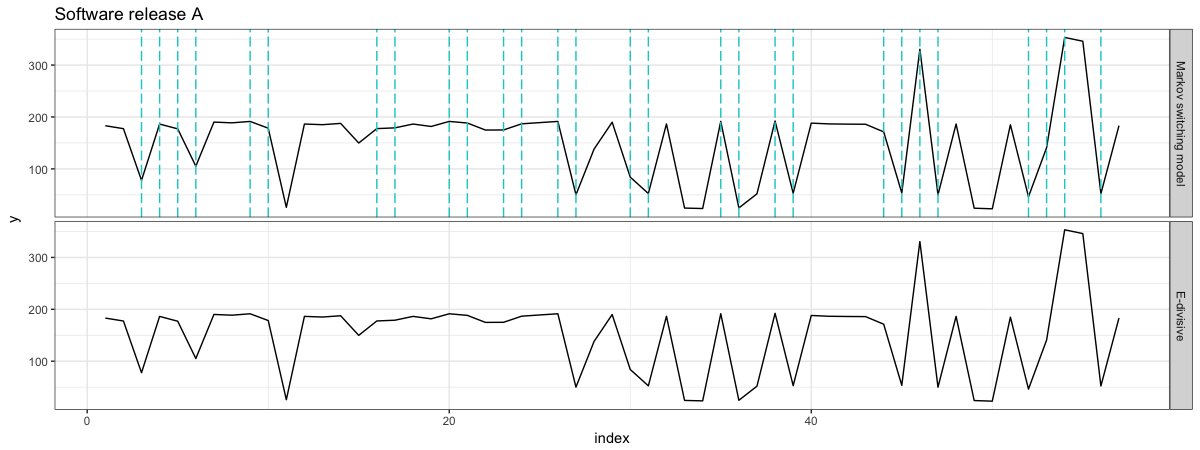
\includegraphics[width=1\linewidth]{compare_L16A}
\caption{Top: Results from the Markov switching model, Bottom: The change point locations from the E-divisive}
\end{figure}

\end{frame}
%------------------------------------------------
\begin{frame}
Real data: Software release B

\begin{itemize}
\item E-divisive method detects change-points at 130, 135, 153, and 170
\end{itemize}

\begin{figure}
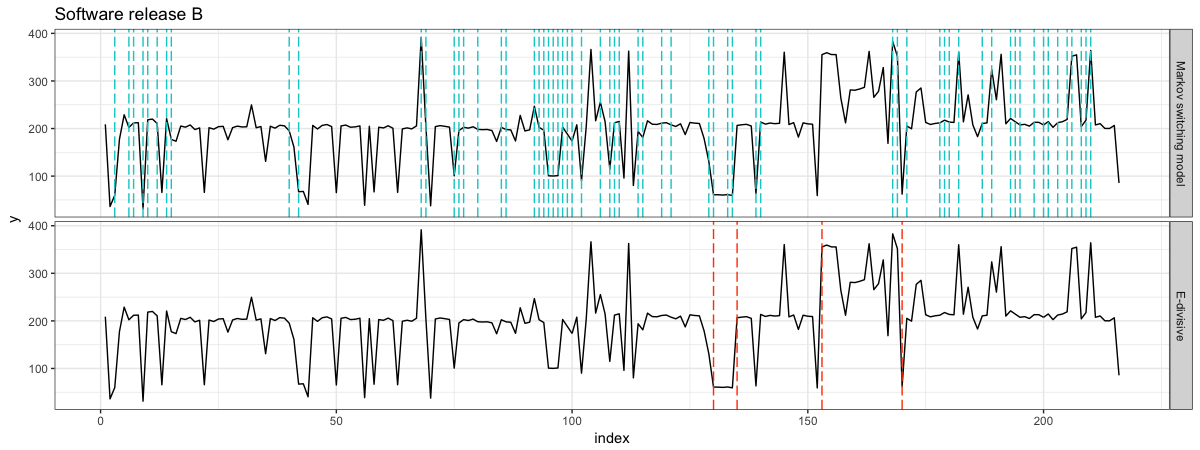
\includegraphics[width=1\linewidth]{compare_L16B}
\caption{Top: Results from the Markov switching model, Bottom: The change point locations from the E-divisive}
\end{figure}

\end{frame}
%------------------------------------------------
\begin{frame}
Real data: Software release C

\begin{itemize}
\item E-divisive method detects change-point at 9, 77, 82, and 105
\end{itemize}

\begin{figure}
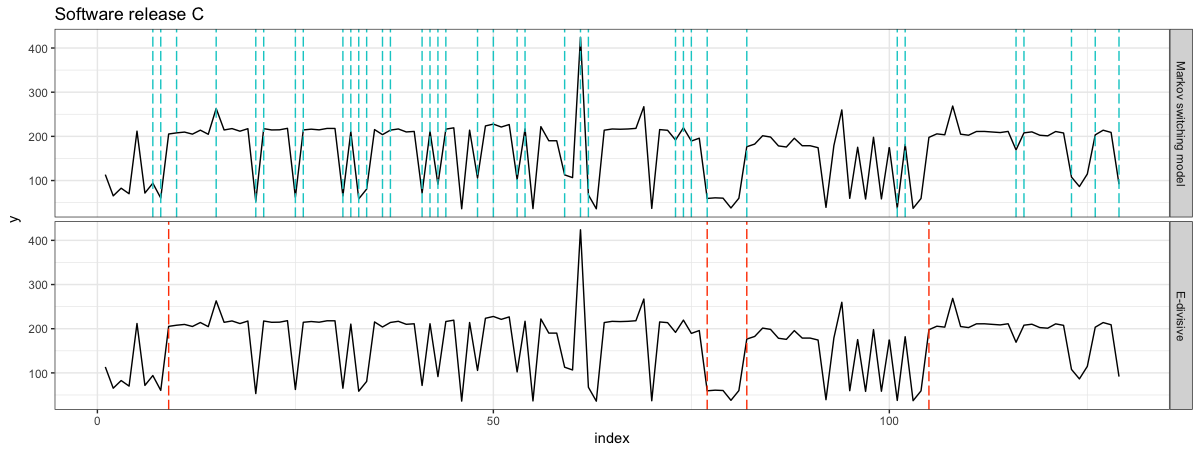
\includegraphics[width=1\linewidth]{compare_L17A}
\caption{Top: Results from the Markov switching model, Bottom: The change point locations from the E-divisive}
\end{figure}
\end{frame}

%------------------------------------------------
\subsection{State inference}
\begin{frame}
Software release A
\pause

\begin{itemize}
\item State 1: Degradation
%\item State 2: Improvement
%\item State 3: Steady
\end{itemize}

\begin{figure}
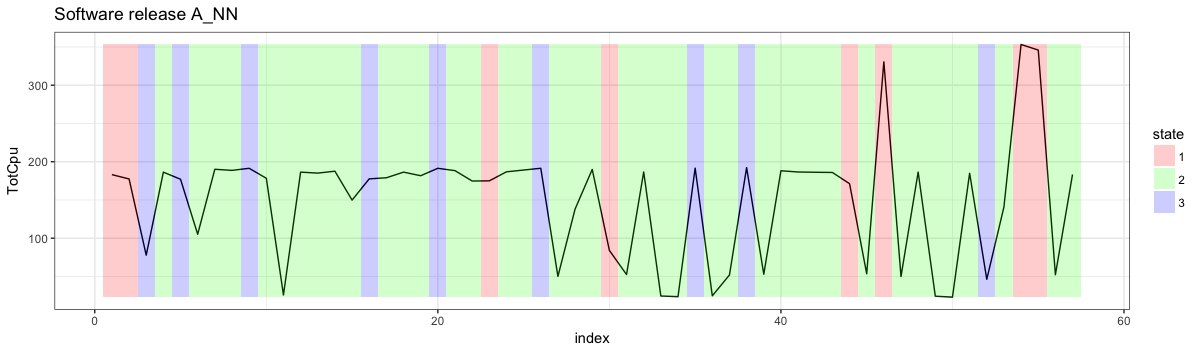
\includegraphics[width=1\linewidth]{L16A_NN1}
\caption{The CPU utilization showing the periods where the observation is in the specific state.}
\end{figure}

\end{frame}

%------------------------------------------------
\begin{frame}
Software release B

\begin{itemize}
\item State 1: Degradation
%\item State 2: Improvement
%\item State 3: Steady
\end{itemize}

\begin{figure}
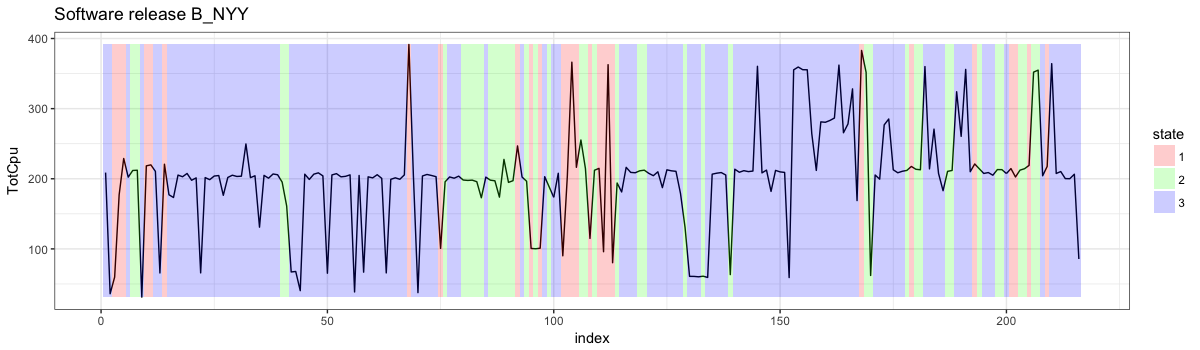
\includegraphics[width=1\linewidth]{L16B_NYY1}
\caption{The CPU utilization showing the periods where the observation is in the specific state.}
\end{figure}

\end{frame}

%------------------------------------------------
\begin{frame}
Software release C

\begin{itemize}
\item State 1: Degradation
%\item State 2: Improvement
%\item State 3: Steady
\end{itemize}

\begin{figure}
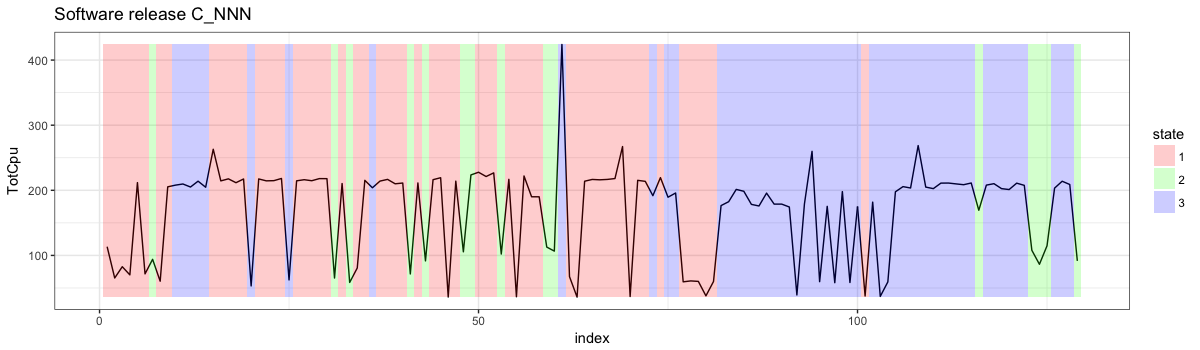
\includegraphics[width=1\linewidth]{L17A_NNN1}
\caption{The CPU utilization showing the periods where the observation is in the specific state.}
\end{figure}

\end{frame}

%------------------------------------------------
\subsection{Test environment}
\begin{frame}[fragile]
Effects of test environments (\textit{DuProdName}, \textit{Fdd/Tdd}, and \textit{NumCells}) on the CPU utilization

\begin{itemize}
\item Software release A:

\textit{Fdd/Tdd} and \textit{NumCells}

\item Software release B:

\textit{DuProdName} and \textit{NumCells}

\item Software release C:

\textit{DuProdName} 

\end{itemize}

\begin{comment}
\subsection{State prediction}
\begin{frame}
Software release L16A

\begin{figure}
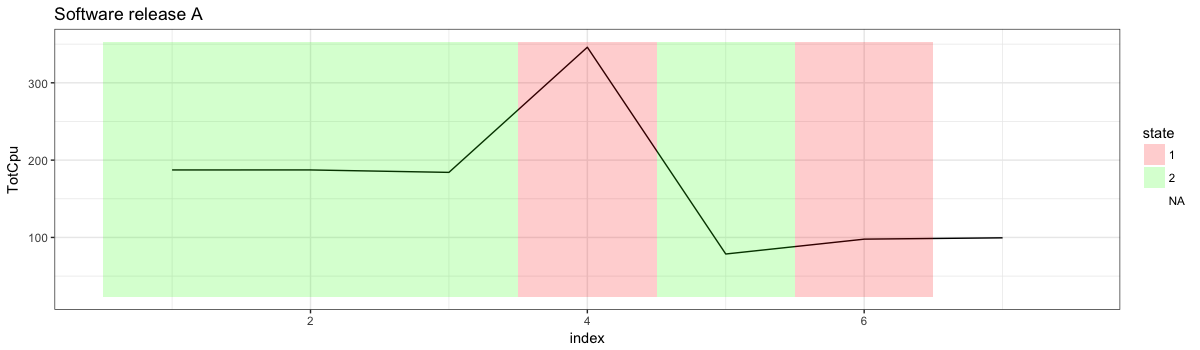
\includegraphics[width=1\linewidth]{predict_L16A1}
\caption{The state prediction of the test set}
\end{figure}
%\end{frame}

%------------------------------------------------
\begin{frame}
Software release L16B

\begin{figure}
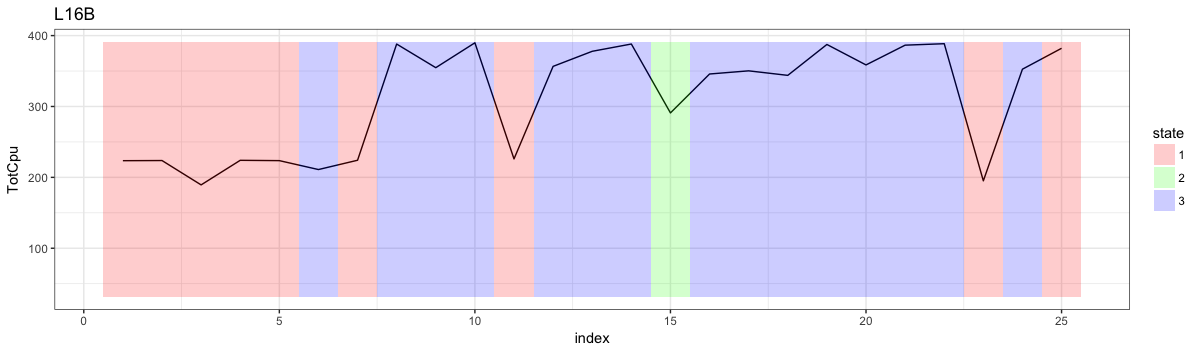
\includegraphics[width=1\linewidth]{predict_L16B1}
\caption{The state prediction of the test set}
\end{figure}
%\end{frame}

%------------------------------------------------
\begin{frame}
Software release L17A

\begin{figure}
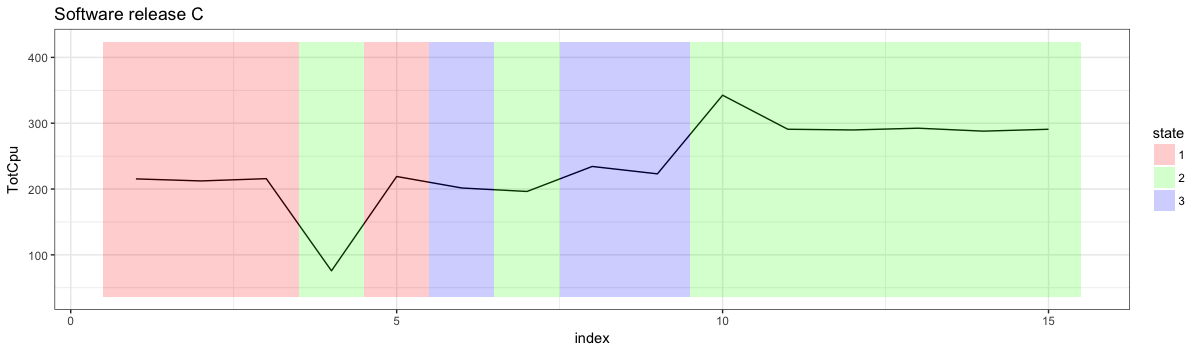
\includegraphics[width=1\linewidth]{predict_L17A1}
\caption{The state prediction of the test set}
\end{figure}
%\end{frame}
\end{comment}
\end{frame}

%------------------------------------------------
%\subsection{Model evaluation}
%\begin{frame}
%The accuracy of the model

%\begin{itemize}
%	\item Simulated Dataset 1: 0.96
%	\item Simulated Dataset 2: 0.80
%\end{itemize}
%\end{frame}
%------------------------------------------------
\section{Conclusion}
\subsection{Conclusion}
\begin{frame}
\begin{itemize}
\item Markov switching model is able to identify any changes between states rather well, despite some false alarms and missed detections
\item E-divisive method  is less powerful as it can detect fewer changes and failed to detect many changes

$\rightarrow$ the method only take into account the value of the CPU utilization

\item Both methods could be used together to confirm the state change
\end{itemize}
\end{frame}

%------------------------------------------------
\subsection{Future work}
\begin{frame}
%\frametitle{Future work}
\begin{itemize}
\item Require more extensive data
\item Consider on the other performance metrics (e.g.,memory usage and latency) 
\item Apply the Markov switching model to each QA Capacity test case type (i.e., one model for one type of test case)
\item Normalize feature set by introducing \textit{weight} parameters
\item Use semi-supervised learning algorithm if some test cases are labeled with state

$\rightarrow$ combining clustering-based and classification-based methods 
\end{itemize}
\end{frame}

%------------------------------------------------
\subsection{References}
\begin{frame}
%\frametitle{References}
\footnotesize{
\begin{thebibliography}{99} % Beamer does not support BibTeX so references must be inserted manually as below
\bibitem[Hamilton, 1989]{p1} James D Hamilton (1989)
\newblock A new approach to the economic analysis of nonstationary time series and the business cycle
\newblock \emph{Econometrica: Journal of the Econometric Society}, pages 357-384.
\end{thebibliography}

\begin{thebibliography}{99} % Beamer does not support BibTeX so references must be inserted manually as below
\bibitem[Sanchez-Espigares, 2014]{p2} Josep A. Sanchez-Espigares and Alberto Lopez-Moreno (2014)
\newblock MSwM: Fitting Markov Switching Models
\newblock \emph{CRAN R}.
\end{thebibliography}

\begin{thebibliography}{99} % Beamer does not support BibTeX so references must be inserted manually as below
\bibitem[James, 2016]{p3} Nicholas A. James and David S. Matteson (2016)
\newblock ecp: Nonparametric Multiple Change Point Analysis of Multivariate Data
\newblock \emph{CRAN R}.
\end{thebibliography}
}
\end{frame}

\end{document} 